\documentclass[14pt, a4paper]{extreport}
\usepackage{import}

\usepackage{float}
\usepackage{graphicx}
\usepackage{subcaption}
\usepackage{fvextra}

\DefineVerbatimEnvironment{verbatim}{Verbatim}{formatcom=\normalfont\normalsize}

\import{../../../lib/}{bridge.sty}

% \title{Squeezes}
% \author{Krysia Gasińska\\ \small{based on Bartek Słupik's ideas}}
\begin{document}
% \maketitle

\begin{titlepage}
    \centering
    \vspace*{2cm}
    {\huge Squeezes\\}
    \vspace{1cm}
    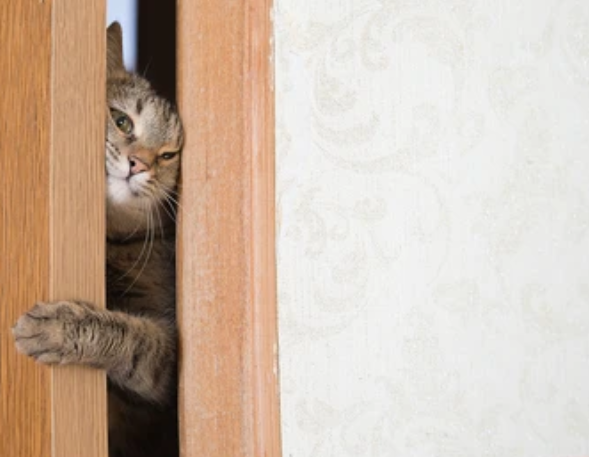
\includegraphics[width=7cm]{./squeezes/cat.png}\\
    \vspace{1cm}
    {\large Krysia Gasińska
    \small{\\
    based on Bartek Słupik's ideas
    }
    }
\end{titlepage}

\section*{Automatic Squeeze}

Oświęcim, 14.09.2024, Turniej o Puchar Prez. Oś., board 26, 4\spades{}S+1
\vspace{0.7cm}

\begin{figure}[H]
    \centering
    \begin{subfigure}{0.4\textwidth}
        \centering
        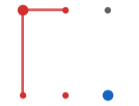
\includegraphics[scale=0.7]{./squeezes/automatic.png}
    \end{subfigure}
    \begin{subfigure}{0.4\textwidth}
        \centering
        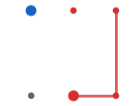
\includegraphics[scale=0.7]{./squeezes/automatic_reverted.png}
    \end{subfigure}
\end{figure}

\handdiagramv{\vhand{KJ932}{Q}{K87}{AKQ2}}
        {\vhand{6}{J94}{QJ632}{J975}}
        {\vhand{Q754}{862}{A95}{T84}}
        {\vhand{AT8}{A{\color{red}K}T753}{T4}{63}}
        {}
\hspace{6.1cm}\clubs{}A\hspace{0.4cm}\clubs{}2\hspace{0.4cm}\diams{}7 
\vspace{-0.4cm}
\begin{figure}[H]
    \centering
    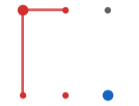
\includegraphics[scale=0.7]{./squeezes/automatic.png}
\end{figure}
\vspace{-0.9cm}
\hspace{6.1cm}\clubs{}4\hspace{0.4cm}\diams{5}\hspace{0.4cm}\spades{Q} 

\vspace{-3cm}
\hspace{10cm}\diams{Q}

\vspace{-0.2cm}
\hspace{10cm}\clubs{J9}

\newpage
\section*{Positional Squeeze}

Warsaw, 18.08.2024, Grand Prix Warszawy, board 5, 6\ntx{}S+1

\vspace{0.7cm}
\begin{figure}[H]
    \centering
    \begin{subfigure}{0.4\textwidth}
        \centering
        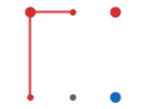
\includegraphics[scale=0.7]{./squeezes/positional.png}
    \end{subfigure}
    \begin{subfigure}{0.4\textwidth}
        \centering
        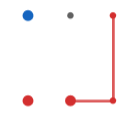
\includegraphics[scale=0.7]{./squeezes/positional_reverted.png}
    \end{subfigure}
\end{figure}

\handdiagramv{\vhand{A32}{KQ}{JT643}{543}}
        {\vhand{K964}{953}{Q5}{JT97}}
        {\vhand{QJ}{AJ6}{AK97}{AKQ6}}
        {\vhand{T875}{T{\color{red}8}742}{82}{82}}
        {}

\vspace{0.3cm}

\hspace{6.3cm}\diams{}J\hspace{0.4cm}\spades{}3\hspace{0.4cm}\clubs{}5 
\vspace{-0.5cm}
\begin{figure}[H]
    \centering
    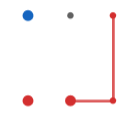
\includegraphics[scale=0.7]{./squeezes/positional_reverted.png}
\end{figure}
\vspace{-0.9cm}
\hspace{6.3cm}\spades{}Q\hspace{0.4cm}\clubs{A}\hspace{0.4cm}\clubs{6} 

\vspace{-3cm}
\hspace{10cm}\spades{K}

\vspace{-0.2cm}
\hspace{10cm}\clubs{JT}

\newpage
\section*{T--Double Squeeze}

7\spades{}S=

\vspace{0.7cm}
\begin{figure}[H]
    \centering
    \begin{subfigure}{0.4\textwidth}
        \centering
        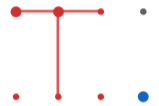
\includegraphics[scale=0.7]{./squeezes/double_T.png}
    \end{subfigure}
    \begin{subfigure}{0.4\textwidth}
        \centering
        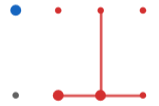
\includegraphics[scale=0.7]{./squeezes/double_T_reverted.png}
    \end{subfigure}
\end{figure}

\handdiagramv
        {\vhand{KQ53}{32}{AK9}{AK65}}
        {\vhand{42}{86}{QT653}{Q932}}
        {\vhand{AJT986}{AKJ}{J82}{8}}
        {\vhand{{\color{red}7}}{QT9754}{74}{JT74}}
        {}

\vspace{0.3cm}

\hspace{5.7cm}\clubs{A}\hspace{0.3cm}\clubs{K}\hspace{0.3cm}\clubs{6}\hspace{0.3cm}\clubs{5}
\vspace{-0.5cm}
\begin{figure}[H]
    \centering
    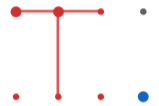
\includegraphics[scale=0.7]{./squeezes/double_T.png}
\end{figure}
\vspace{-0.9cm}
\hspace{5.8cm}\hearts{J}\hspace{0.4cm}\clubs{8}\hspace{0.4cm}\diams{J}\hspace{0.4cm}\spades{6}

\vspace{-3cm}
\hspace{3.5cm}\hearts{Q}\hspace{6.5cm}\diams{Q}

\vspace{-0.2cm}
\hspace{3.5cm}\clubs{JT7}\hspace{6cm}\clubs{Q93}

\newpage
\section*{R--Double Squeeze}

7\ntx{}S=

\vspace{0.7cm}
\begin{figure}[H]
    \centering
    \begin{subfigure}{0.4\textwidth}
        \centering
        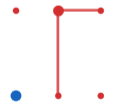
\includegraphics[scale=0.7]{./squeezes/double_R.png}
    \end{subfigure}
    \begin{subfigure}{0.4\textwidth}
        \centering
        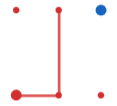
\includegraphics[scale=0.7]{./squeezes/double_R_reverted.png}
    \end{subfigure}
\end{figure}

\handdiagramv
        {\vhand{AQ5}{J875}{Q62}{A32}}
        {\vhand{76}{9}{JT954}{QT865}}
        {\vhand{KJ432}{AK}{AK83}{K4}}
        {\vhand{{\color{red}T}98}{QT6432}{7}{J97}}
        {}

\vspace{0.3cm}

\hspace{6.3cm}\hearts{J}\hspace{0.4cm}\clubs{A}\hspace{0.4cm}\clubs{3}
\vspace{-0.5cm}
\begin{figure}[H]
    \centering
    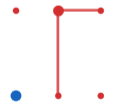
\includegraphics[scale=0.7]{./squeezes/double_R.png}
\end{figure}
\vspace{-0.9cm}
\hspace{6.3cm}\spades{4}\hspace{0.4cm}\clubs{4}\hspace{0.4cm}\diams{8} 

% \newpage
% \section*{X--Double Squeeze}

% ---

% \vspace{0.7cm}
% \begin{figure}[H]
%     \centering
%     \begin{subfigure}{0.4\textwidth}
%         \centering
%         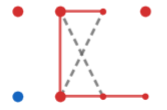
\includegraphics[scale=0.7]{./squeezes/double_X.png}
%     \end{subfigure}
%     \begin{subfigure}{0.4\textwidth}
%         \centering
%         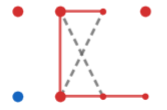
\includegraphics[scale=0.7]{./squeezes/double_X.png}
%     \end{subfigure}
% \end{figure}

% \handdiagramv
%         {\vhand{}{}{}{}}
%         {\vhand{}{}{}{}}
%         {\vhand{}{}{}{}}
%         {\vhand{}{}{}{}}
%         {}

% \vspace{0.3cm}

% \hspace{6.3cm}\diams{}J\hspace{0.4cm}\spades{}3\hspace{0.4cm}\clubs{}5 
% \vspace{-0.5cm}
% \begin{figure}[H]
%     \centering
%     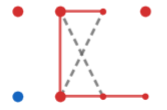
\includegraphics[scale=0.7]{./squeezes/double_X.png}
% \end{figure}
% \vspace{-0.9cm}
% \hspace{6.3cm}\spades{}Q\hspace{0.4cm}\clubs{A}\hspace{0.4cm}\clubs{6} 

% \newpage
% \section*{Criss-Cross Squeeze}

% ---

% \vspace{0.7cm}
% \begin{figure}[H]
%     \centering
%     \begin{subfigure}{0.4\textwidth}
%         \centering
%         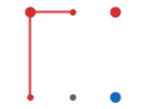
\includegraphics[scale=0.7]{./squeezes/positional.png}
%     \end{subfigure}
%     \begin{subfigure}{0.4\textwidth}
%         \centering
%         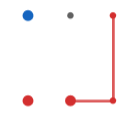
\includegraphics[scale=0.7]{./squeezes/positional_reverted.png}
%     \end{subfigure}
% \end{figure}

% \handdiagramv
%         {\vhand{}{}{}{}}
%         {\vhand{}{}{}{}}
%         {\vhand{}{}{}{}}
%         {\vhand{}{}{}{}}
%         {}

% \vspace{0.3cm}

% \hspace{6.3cm}\diams{}J\hspace{0.4cm}\spades{}3\hspace{0.4cm}\clubs{}5 
% \vspace{-0.5cm}
% \begin{figure}[H]
%     \centering
%     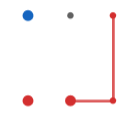
\includegraphics[scale=0.7]{./squeezes/positional_reverted.png}
% \end{figure}
% \vspace{-0.9cm}
% \hspace{6.3cm}\spades{}Q\hspace{0.4cm}\clubs{A}\hspace{0.4cm}\clubs{6} 

% \newpage
% \section*{Trump Squeeze}

% ---

% \vspace{0.7cm}
% \begin{figure}[H]
%     \centering
%     \begin{subfigure}{0.4\textwidth}
%         \centering
%         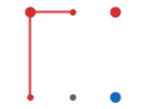
\includegraphics[scale=0.7]{./squeezes/positional.png}
%     \end{subfigure}
%     \begin{subfigure}{0.4\textwidth}
%         \centering
%         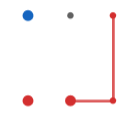
\includegraphics[scale=0.7]{./squeezes/positional_reverted.png}
%     \end{subfigure}
% \end{figure}

% \handdiagramv
%         {\vhand{}{}{}{}}
%         {\vhand{}{}{}{}}
%         {\vhand{}{}{}{}}
%         {\vhand{}{}{}{}}
%         {}

% \vspace{0.3cm}

% \hspace{6.3cm}\diams{}J\hspace{0.4cm}\spades{}3\hspace{0.4cm}\clubs{}5 
% \vspace{-0.5cm}
% \begin{figure}[H]
%     \centering
%     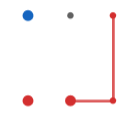
\includegraphics[scale=0.7]{./squeezes/positional_reverted.png}
% \end{figure}
% \vspace{-0.9cm}
% \hspace{6.3cm}\spades{}Q\hspace{0.4cm}\clubs{A}\hspace{0.4cm}\clubs{6} 

\newpage
\section*{Non-simultanous double squeeze}
[adapted] Warsaw, 31.05.2024, Memoriał J. Gresia, board 18, 6\ntx{}S+1

\vspace{0.7cm}
\begin{figure}[H]
    \centering
    \begin{subfigure}{0.4\textwidth}
        \centering
        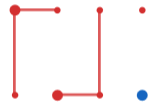
\includegraphics[scale=0.7]{./squeezes/nonsim-double.png}
    \end{subfigure}
    \begin{subfigure}{0.4\textwidth}
        \centering
        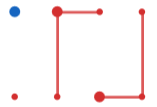
\includegraphics[scale=0.7]{./squeezes/nonsim-double-reverted.png}
    \end{subfigure}
\end{figure}

\handdiagramv
        {\vhand{74}{KQ65}{T53}{KJ94}}
        {\vhand{QJT53}{32}{874}{Q32}}
        {\vhand{A8}{A84}{AKQJ92}{A6}}
        {\vhand{K962}{{\color{red}J}T97}{6}{T875}}
        {}

\vspace{0.3cm}

\hspace{5.8cm}\hearts{K}\hspace{0.4cm}\hearts{5}\hspace{0.4cm}\spades{4}\hspace{0.4cm}\clubs{J}
\vspace{-0.4cm}
\begin{figure}[H]
    \centering
    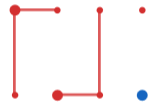
\includegraphics[scale=0.7]{./squeezes/nonsim-double.png}
\end{figure}
\vspace{-0.9cm}
\hspace{5.8cm}\hearts{4}\hspace{0.4cm}\spades{A}\hspace{0.4cm}\spades{8}\hspace{0.4cm}\diams{2}

\vspace{-3cm}
\hspace{3.5cm}\spades{K2}\hspace{6cm}\spades{QJT}

\vspace{-0.2cm}
\hspace{3.5cm}\hearts{T9}\hspace{6cm}\clubs{Q}

\newpage
\section*{Non-simultanous alternative squeeze}
Warsaw, 31.05.2024, Memoriał J. Gresia, board 18, 6\ntx{}S+1

\handdiagramv
        {\vhand{J4}{KQ65}{T53}{KJ94}}
        {\vhand{T8753}{32}{874}{Q32}}
        {\vhand{AQ}{A84}{AKQJ92}{A6}}
        {\vhand{K962}{{\color{red}J}T97}{6}{T875}}
        {}

\vspace{0.3cm}

\hspace{5.8cm}\hearts{K}\hspace{0.4cm}\hearts{5}\hspace{0.4cm}\spades{J}\hspace{0.4cm}\clubs{J}
\vspace{-0.4cm}
\begin{figure}[H]
    \centering
    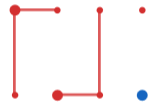
\includegraphics[scale=0.7]{./squeezes/nonsim-double.png}
\end{figure}
\vspace{-0.9cm}
\hspace{5.8cm}\hearts{4}\hspace{0.4cm}\spades{A}\hspace{0.4cm}\spades{Q}\hspace{0.4cm}\diams{2}

\vspace{-3cm}
\hspace{3.5cm}\spades{K2}\hspace{6cm}\spades{T87}

\vspace{-0.2cm}
\hspace{3.5cm}\hearts{T9}\hspace{6cm}\clubs{Q}

\vspace{2cm}
The difference is, only one opponent holds the \spades menace, but either one can hold it.

\end{document}